\section{Increment 1}

\subsection{Introduction}
At first, we must know the software is a scientific computation platform. It is composed of two main parts. The first part is made of a
formalization module and a solving strategy one. This part is the intelligence of the software. In front of that, the second part which
manage XML data, has the same structure that the first part.\\

This document aims to present the tests done to validate the functioning of the platform.\\
In this document you will find two main parts :
\begin{itemize}
        \item a File part, which defines the development strategy used and the satisfaction criterions.
        \item a Result part, which explain the results of the tests and analyze them.
\end{itemize}


\subsection{Tests file}
This chapter defines in detail, all the tests used, the adopted development strategy, and the satisfaction criterions.

\subsubsection{Introduction}
The acceptance tests have been realized during the development of the plugin which allowed to simule the fall of a ball on a rigid plan.
It is a very simple example, but it allows to validate the stages order of the simulation, the functioning of mechanisms for saving and
loading \ac{xml} data as well as the plugins' mechanism of the platform.

\subsubsection{Testing strategy}
The test takes place in the following way : we read an input data file; file written with the \ac{moad}, then we do computations on the
desired number of steps. The results are validated by the \ac{moad}.

\subsubsection{Satisfaction criterions}
The acceptance tests are validated by the person in charge for the tests, for the quality and by the \ac{moad}. The acceptance tests are
based on the requirements expressed by the customer in the \ac{srd}.\\
The tests detailled in this document are based in the \ac{op}, which is the milestone until june 2004.
%\begin{ndr}
%continuer ce doc en precisant les differents objectifs de septembre et d'avril.
%\end{ndr}

\subsubsection{Development of the tests}
(Work breakdown structure.3612)\\
%\subsubsection{XML input file}
\paragraph{XML input file}
(Work breakdown structure.3611.1, 3611.2)\\
It consists in the description of 2 Lagrangian systems :a ball and a rigid plan. They are represented as \textit{Lagrangian Time Invariant Dynamic Systems}.\\
This file is available in the appendices of this document.

%\subsubsection{Ball simulation test}
\paragraph{Ball simulation test}
(Work breakdown structure.3612.1)\\
For this test, a plugin : BallPLugin.c, has been developped to calculate specific functions of this problem (calculation of inertia, of
the mass and external forces).


%======report to put somewhere else=============

%\section{Acceptance tests report}
%The acceptance test has been run, the file \ref{BouncingBall_TIDS.xml} has been read and computations has been done to make a ball
%bouncing on a rigid plan. On the \ref{acceptanceTest} we can see the position of the ball, the velocity of this ball
%and the force that make the ball bouncing when it touch the floor.
%\begin{figure}[!hbp]
%\begin{center}
%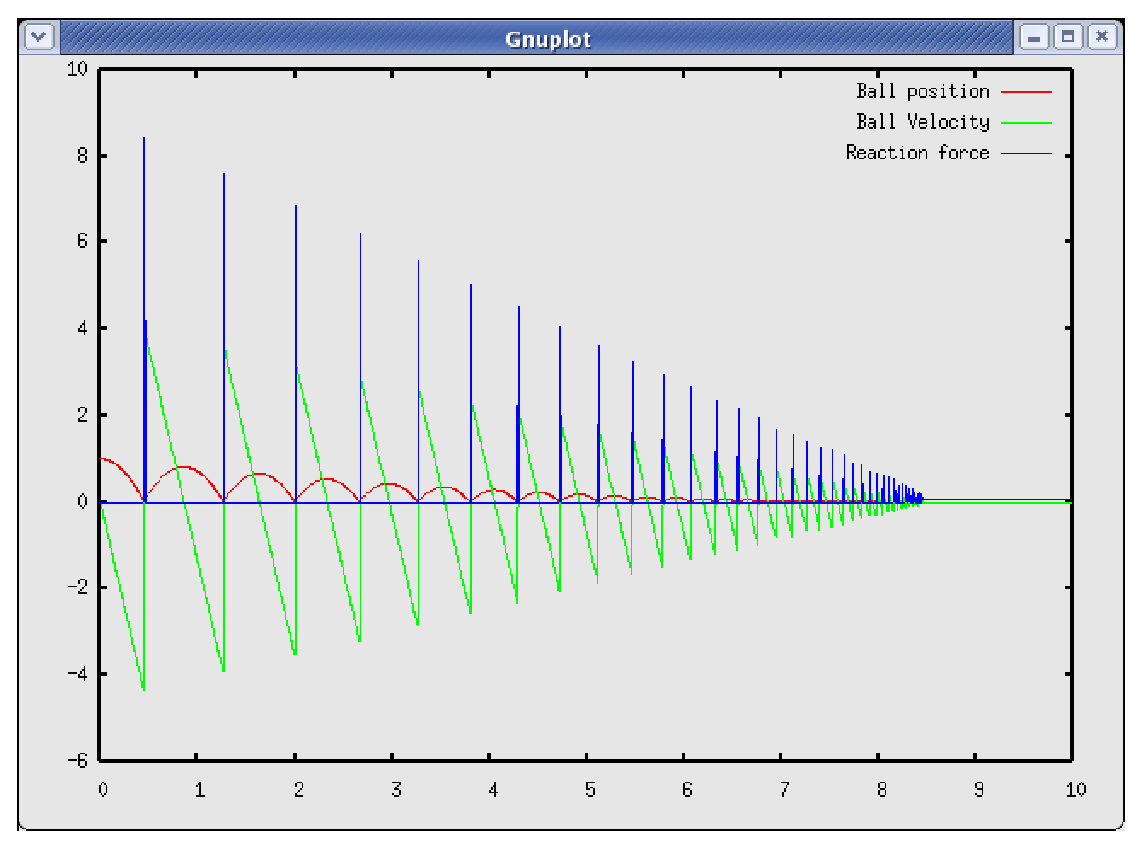
\includegraphics[scale=0.80]{figure/acceptanceTest.ps}
%\caption{Results of the bouncing ball test}
%\label{acceptanceTest}
%\end{center}
%\end{figure}


%===================
%\appendix
%\newpage
%\chapter{\ac{xml} input file of the bouncing ball test}
%\label{BouncingBall_TIDS.xml}
%\verbatiminput{BouncingBall_TIDS.xml}
